%Need to include: ``in combination with local improvement heuristics \citep{schwerin1997} and metaheuristic methods such as tabu search \citep{alvim2004}''.
%-------------------------

\documentclass[a4paper,11pt]{article}
%---- PREAMBLE ----%

% Allows separate files to be used in the main file
\usepackage{subfiles}

% Algorithms
\usepackage{algorithm}
\usepackage[noend]{algpseudocode}
\renewcommand{\algorithmicrequire}{\textbf{Input:}}
\renewcommand{\algorithmicensure}{\textbf{Output:}}
\newcommand{\algorithmicbreak}{\State \textbf{break}}
\newcommand{\Break}{\algorithmicbreak}
\renewcommand{\algorithmicreturn}{\State \textbf{return}}
\newcommand{\algorithmicto}{\textbf{ to }}
\newcommand{\To}{\algorithmicto}
\newcommand{\algorithmicrun}{\State \textbf{call }}
\newcommand{\Run}{\algorithmicrun}
\newcommand{\algorithmicoutput}{\textbf{output }}
\newcommand{\Output}{\algorithmicoutput}
\newcommand{\algorithmictrue}{\textbf{true}}
\newcommand{\True}{\algorithmictrue}
\newcommand{\algorithmicfalse}{\textbf{false}}
\newcommand{\False}{\algorithmicfalse}

% Contains advanced math extensions
\usepackage{amsmath}

% Introduces the *proof* environment and the \theoremstyle command
\usepackage{amsthm}

% Adds new symbols to be used in math mode, e.g. \mathbb
\usepackage{amssymb}

% To declare multiple authors
%\usepackage{authblk}

% Provides extra comands as well as optimisation for producing tables
\usepackage{booktabs}
\newcommand{\ra}[1]{\renewcommand{\arraystretch}{#1}}

% Allows customisation of appearance and placements for figures/tables etc.
\usepackage{caption}

% Adds support for arbitrarily-deep nested lists
\usepackage[inline]{enumitem}

%Support for changing size of font in table footnotes
\usepackage{etoolbox}

% Improves the interface for defining floating objects such as figures/tables
\usepackage{float}

\usepackage{fullpage}

% For easy management of document margins and the document page size
%\usepackage[a4paper]{geometry}

% Allows insertion of graphic files within a document
\usepackage{graphicx}

% Manage links within the document or to any URL when you compile in PDF
\usepackage[colorlinks]{hyperref} 
\usepackage[dvipsnames]{xcolor}
%Tikz colours, used in tikz figures only
\colorlet{tBlue}{RoyalBlue!35!Cerulean} %tikz color
\colorlet{tRed}{Red} %tikz color
\definecolor{tGreen}{HTML}{569909} %tikz color
\definecolor{tOrange}{HTML}{FA7602} %tikz color

%Text colours
\colorlet{myRed}{Red!50!OrangeRed}
\definecolor{myOrange}{HTML}{FA7602}
\definecolor{myGreen}{HTML}{569909}
\definecolor{myAqua}{HTML}{00B1BA} %02BEB8
\definecolor{myBlue}{HTML}{0095FF} %00B3FF
\colorlet{myPurple}{Orchid} 
\colorlet{myPink}{Rhodamine!65!Lavender}
\colorlet{myGray}{Gray!90!White}

% The document class `elsarticle` uses the \AtBeginDocument comman to define the colour of all link types as blue, so we use the \AtBeginDocument command again to overwrite the colour settings to the colors we choose. REMEMBER TO REMOVE THIS BEFORE SUBMITTING.
\AtBeginDocument{% 
	\hypersetup{
		linkcolor=myPurple,
		citecolor=myAqua,
		urlcolor=black
	}
} %end of \AtBeginDocument

\newcommand{\intro}[1]{{\color{myOrange}#1}} % \intro{<text>}, makes <text> orange, use to highlight things to do, urgent, or revisit in introduction section

\newcommand{\ahc}[1]{{\color{myBlue}#1}} % \ahc{<text>}, makes <text> blue, use to highlight things to do, urgent, or revisit in AHC section

\newcommand{\heur}[1]{{\color{myPink}#1}} % \scspp{<text>}, makes <text> pink, use to highlight things to do, urgent, or revisit in SCSPP section

\newcommand{\ea}[1]{{\color{myRed}#1}} % \ea{<text>}, makes <text> red, use to highlight things to do, urgent, or revisit in EA section

\newcommand{\cmsa}[1]{{\color{myGreen}#1}} % \cmsa{<text>}, makes <text> green, use to highlight things to do, urgent, or revisit in CMSA section

\newcommand{\conc}[1]{{\color{myPurple}#1}} % \conc{<text>}, makes <text> purple, use to highlight things to do, urgent, or revisit in Conclusion section

\newcommand{\note}[1]{{\color{myPurple}#1}} % \note{<text>}, makes <text> turquoise, use to highlight things to do, urgent, or revisit in any section


\newcommand{\alert}[1]{{\color{myRed}#1}} % \alert{<text>}, makes <text> red, use to highlight things to do, urgent, or revisit.

\newcommand{\done}[1]{{\color{myGray}#1}} % \done{<text>}, makes <text> gray, use to highlight things that are not required or should be ignored.

\newcommand{\ialert}[1]{{\color{myRed}\item#1}} % \ialert{<text>}, makes <text> a red bullet point, use for bullet points of things to do, urgent, or revisit.

\newcommand{\idone}[1]{{\color{myGray}\item#1}} % \idone{<text>}, makes <text> a gray bullet point, use for bullet points that have been completed, that are not required or should be ignored.

\renewcommand{\idone}[1]{} % hides all \idone bullet points

% Successor of amsmath
\usepackage{mathtools}

\usepackage{multirow}

% No indentation, space between paragraphs
%\usepackage{parskip}

\usepackage{natbib}

%Include standalone .tex files
\usepackage{standalone}

% Define multiple floats (figures/tables) within one environment with individual captions 1a, 1b etc
\usepackage{subcaption}

\usepackage{tabularx}

\usepackage{threeparttable}
\appto\TPTnoteSettings{\footnotesize} % Change font size of table footnotes to footnotesize

\usepackage{tikz}

\usepackage{wrapfig}

\DeclarePairedDelimiter{\floor}{\lfloor}{\rfloor}
\DeclarePairedDelimiter{\ceil}{\lceil}{\rceil}

%Theorem style
\theoremstyle{plain}% default
\newtheorem{theorem}{Theorem}
%\newtheorem{corollary}{Corollary}
\newtheorem{definition}{Definition}

%\theoremstyle{definition}
%\newtheorem{definition}{Definition}
%\newtheorem{proposition}{Proposition}
%\newtheorem{exmp}{Example}[section]
\begin{document}
	
\title{A Survey on Packing Problems with Ordering and Orientation Constraints}
\author{Asyl L. Hawa}
\date{}
\maketitle
		
\noindent In this chapter, we start by providing a brief overview to computational complexity, which allows us to assess the difficulty of various combinatorial optimisation problems. We then introduce the one-dimensional bin packing problem (BPP) and discuss the methods that have been used to solve the problem by reviewing relevant literature, before exploring alternative packing problems related to the BPP. The Score-Constrained Packing Problem (SCPP) is also examined and compared to the various packing problems highlighted throughout the chapter.

%-------------------------------------------------------------------------------------
\section{Introduction}
\label{sec:intro}
\begin{comment}
\begin{itemize}[itemsep=-0.4em, leftmargin=*]
	\item Cutting and Packing problems, every day problems, applications
	\item Aim/task of general C+P problems
	\item 1DBPP classical problem, aim, most well-known
	\item Formal 1DBPP definition and notation
	\item ILP formulation
	\item Washcer typology
	\item Decision vs optimisation variants of 1DBPP
	\item Complexity of 1DBPP, NP-hard/complete reducing partition problem
	\item Grouping problems and formulation
	\item 1DBPP as GCP/Timetabling problem?
	\item History of 1DBPP, \citet{kantorovich1960} (from the 30s)
	\item ODMGPs, OIMGPs and examples
	\item Task is minimising the objective function, i.e. number of bins
	\item Figure 1DBPP problem instance and solution
	\item Multidimensional versions?
\end{itemize}
\end{comment}

\noindent \lit{From sorting belongings into boxes when moving house to loading goods into delivery vans, packing problems occur frequently -- yet often unknowingly -- in our everyday lives. Naturally, in order to reduce costs and prevent waste, the aim of the majority of such problems is to pack all of the ``items'' efficiently into the ``bins'' so as to make use of all of the space provided, whilst also attempting to minimise the number of bins required. In some cases this also has an environmental benefit, reducing vehicle emissions and the demand for materials. The conditions for each packing problem can vary. For example, when moving house it is often desirable to pack items from the same room or category into the same set of boxes, whereas supermarkets may choose to organise goods into vehicles in the order they are to be delivered to customers. In this thesis, we focus on a specific packing problem with conditions involving the order and orientation of the items in the bins: the Score-Constrained Packing Problem (SCPP).}

\noindent One particular class of grouping problem with applications in the material and construction industries are cutting and packing problems. These problems involve cutting items from stock material or packing items into bins subject to specific constraints. Perhaps the most well-known of these problems is the one-dimensional bin packing problem (BPP).

\begin{definition}
	Given a set $\mathcal{I}$ of $n$ rectangular items of varying widths $w_i \in \mathbb{Z}^+$ and equal height $H>0$ for all items $i \in \mathcal{I}$, the \emph{one-dimensional bin packing problem (BPP)} involves packing all items in $\mathcal{I}$ into the fewest number of $H \times W$ bins such that no bin is overfilled.
	\label{defn:bpp}
\end{definition}

\noindent The one-dimensional bin packing problem is a classical combinatorial optimisation problem originating back to the 1930s \citep{kantorovich1960}. The problem requires the items in $\mathcal{I}$ to be grouped into subsets $\mathcal{S} = \{S_1,\dotsc,S_k\}$ of bins with the aim of minimising the number of bins $k$. For this problem, a bin $S_j$ is feasible if the total widths of all the items in $S_j$ does not exceed the bin capacity $W$; that is, $A(S_j) = \sum_{i \in S_j} w_i \leq W$. \lit{A basic lower bound for the fewest number of bins $k$ in a solution is the theoretical minimum, which can be calculated in $O(n)$ time \citep{martello1990l}:}

\begin{equation}
\lit{t = \ceil*{\frac{\sum_{i=1}^{n} w_i}{W}}.}
\label{eq:tmin}
\end{equation}
%\vspace{0.5mm}

\noindent Figure~\ref{fig:bppsoln} depicts an example instance $\mathcal{I}$ of 10 items for the BPP to be packed into bins of capacity $W = 1000$ along with a feasible solution comprising three bins. \lit{As the theoretical minimum for this problem instance is $t=3$, the solution is in fact optimal.} 

\begin{figure}[h!]
	\centering	
	%\hspace{-7mm}
	\begin{subfigure}[b]{0.50\textwidth}
		\includestandalone[width=\textwidth]{figures/bppitems}
		\vspace{0.01mm}
		\caption{$\mathcal{I}$}
		\label{fig:bppitems}
	\end{subfigure} \hspace{1mm}
	\begin{subfigure}[b]{0.47\textwidth}
		\includestandalone[width=\textwidth]{figures/bpp}
		\vspace{0.01mm}
		\caption{Solution for $\mathcal{I}$}
		\label{fig:bpp}
	\end{subfigure}
	\caption{(a) An example instance $\mathcal{I}$ of the BPP comprising 10 items; and (b) a feasible solution for the instance using three bins of capacity $W = 1000$. The remaining space in each bin is shaded in grey.\lit{ As the theoretical minimum $t=3$, the solution is optimal.}}	
	\label{fig:bppsoln}
\end{figure}

\noindent There also exists a decision variant of the problem, which consists in determining whether a given set of items $\mathcal{I}$ can be packed into \lit{exactly/less than} $k$ bins \lit{(yes or no)}. Clearly, by repeating the decision variant of the problem and reducing the value of $k$ we can obtain a solution to the corresponding optimisation problem, i.e. the minimum number of bins required to pack all items feasibly.


The BPP can be formulated as the following integer linear program:
\begin{subequations}
	\begin{align}
	\text{minimise  } &\qquad \sum_{j=1}^{n} y_j & \label{eq:objfnbpp}\\[3pt]
	\text{subject to  } &\qquad \sum_{i = 1}^{n} w_i x_{ij} \leq W y_j & j = 1,\dotsc,n \label{eq:capacitybpp} \\[3pt]
	&\qquad \sum_{j=1}^{n} x_{ij} = 1 &i = 1,\dotsc,n \label{eq:nointersectbpp} \\[3pt]
	&\qquad y_j \in \{0,1\} &j = 1,\dotsc,n \label{eq:binarybppy} \\[3pt]
	&\qquad x_{ij} \in \{0,1\} &i,j = 1,\dotsc,n \label{eq:binarybppx}
	\end{align}
\end{subequations}
\begin{alignat*}{2}
& \begin{aligned} & 
y_j = 
\begin{cases}
1 & \text{if bin } j \text{ is used} \\
0 & \text{otherwise} \\
\end{cases} \\
\end{aligned}
& \hskip 2em 
& \begin{aligned} & 
x_{ij} = 
\begin{cases}
1 & \text{if item } i \text{ is packed into bin } j \\
0 & \text{otherwise.} \\
\end{cases} \\
\end{aligned}
\end{alignat*}
\vspace{3pt}

\noindent The objective \ref{eq:objfnbpp} is to minimise the number of bins of capacity $W$ used to pack the items. Constraint~\ref{eq:capacitybpp} ensures that the bins used in the solution are not overfilled, whilst Constraint~\ref{eq:nointersectbpp} states that each item must be packed into exactly one of the bins in the solution. The final two constraints restrict the variables $x_{ij}$ and $y_j$ to the integers 0 and 1.

Derived from the one-dimensional bin packing problem are the two-dimensional \citep{lodi2002} and three-dimensional \citep{martello2000} bin packing problems. The BPP has a variety of real world applications, such as assigning advertisements to programme breaks in television broadcasting \citep{brown1971}, allocating memory in computer network designs \citep{chandra1978}, scheduling tasks on multiple processors \citep{coffman1978, vandevel1991}, and packing items into containers with size or weight capacity constraints \citep{eilon1971, hung1978}.

\subsection{Computational Complexity of the Bin Packing Problem}
\label{sub:complexitybpp}

\noindent The partition problem asks the question: ``given a set $S$ of positive integers, can $S$ be partitioned into two subsets $S_1$ and $S_2$ such that the sum of the elements in $S_1$ is equal to the sum of the elements in $S_2$?'' This decision problem is known to be NP-complete, and is in fact one of \citeauthor{karp1972}'s original 21 NP-complete problems (1972). As discussed in Section~\ref{sec:complexity}, by reducing the partition problem to the BPP we are able to show that the BPP is also NP-complete.

\begin{theorem}
	Given an instance $\mathcal{I}$ of the BPP, the problem of deciding whether there exists a solution to $\mathcal{I}$ comprising two bins is NP-complete.
	\label{thm:bppnpcomplete}
\end{theorem}

\begin{proof}
	We reduce the partition problem, which we know to be NP-complete, to the above bin packing problem. Given an instance $S = \{s_1,\dotsc,s_n\}$ of the partition problem, consider the instance $\mathcal{I} = \{w_1,\dotsc,w_n\}$ of the BPP, where
	\[
	w_i = \frac{2s_i}{\sum_{j=1}^n s_j} \hspace{5mm} \forall \hspace{1mm} i = 1,\dotsc,n.
	\]
	Clearly, there exists a solution for the BPP using two bins if and only if there exists a subset $S_1 \subseteq \{1,\dotsc,n\}$ such that $\sum_{i\in S_1} s_i = \sum_{i \notin S_1} s_i$.
\end{proof}		

\noindent As the decision variant of the BPP is NP-complete, it follows that the optimisation variant of the BPP, provided in Definition~\ref{defn:bpp}, is NP-hard \citep{garey1978,garey1979}.


%-------------------------------------------------------------------------------------

\section{Heuristics for the Bin Packing Problem}
\label{sec:heurbpp}

\noindent As the BPP is NP-hard, under the generally accepted assumption that P$\neq$NP we cannot hope to find an optimal solution in polynomial-time for all instances of the BPP. Consequently, much research has been devoted to developing algorithms that run in polynomial-time that produce near-optimal solutions, such as heuristics and approximation algorithms. Heuristics aim to produce feasible solutions by trading optimality, accuracy, or precision for speed; thus solutions created by heuristics are not guaranteed to be optimal. Approximation algorithms are heuristics that have the advantage of producing solutions that are provably close to the optimal solution, which makes them much more desirable in theory. It is important to note, however, that the worst-case bounds obtained from approximation algorithms cover all instances of a problem including unusual instances that would not appear in practice, and so it tends to be that heuristics derived from approximation algorithms produce solutions that are much closer to the optimal than suggested by the bounds of the approximation algorithm \citep{williamson2011}.

Let $\mathcal{A}(\mathcal{I})$ denote the number of bins in a solution for an instance $\mathcal{I}$ produced using an approximation algorithm $\mathcal{A}$, and let OPT$(\mathcal{I})$ denote the number of bins in the optimal solution for the instance $\mathcal{I}$. Then, $\mathcal{A}$ has an approximation ratio $c>1$ if for any instance $\mathcal{I}$, $\mathcal{A}(\mathcal{I}) \leq c$OPT$(\mathcal{I}) + b$, where $b$ is a positive constant. Clearly, the goal is to obtain an approximation ratio $c$ that is as close to 1 as possible. However, \citet{vazirani2003} has shown that there cannot exist an approximation algorithm with $c < \frac{3}{2}$ for the BPP unless P=NP.

One of the most well-known heuristics for the BPP is First-Fit (FF), a greedy online algorithm that packs each item, given in some arbitrary order, into the lowest-indexed bin that can feasibly accommodate the item and opening a new bin when required, as shown in Algorithm~\ref{alg:ff}. It is known that there always exists at least one ordering of the items such that FF produces an optimal solution \citep{lewis2009}. 

\begin{algorithm}[h]	
\caption{FF($\mathcal{I}$)}
\label{alg:ff}
\small
\begin{algorithmic}[1]
	\State $A(S_j) \gets 0$ $\forall$ $j=1,\dotsc,|\mathcal{I}|$ \Comment All bins are initially empty
	\State $\mathcal{S} \gets \emptyset$
	\For{$i \gets 1 \To |\mathcal{I}|$}
		\State $j \gets 1$
		\State packed $\gets \False$
		\While{$\Not$ packed}
			\If{$S_j \in \mathcal{S}$}
				\If{$A(S_j) + w_i \leq W$}
					\State $S_j \gets S_j \cup \{i\}$
					\State $A(S_j) \gets A(S_j) + w_i$
					\State packed $\gets \True$
				\Else \hspace{0.2mm} $j \gets j + 1$
				\EndIf
			\ElsIf{$S_j \notin \mathcal{S}$}
				\State $S_j \gets S_j \cup \{i\}$
				\State $A(S_j) \gets A(S_j) + w_i$
				\State $\mathcal{S} \gets \mathcal{S} \cup \{S_j\}$
				\State packed $\gets \True$
			\EndIf
		\EndWhile
	\EndFor	
	\Return $\mathcal{S}$	
\end{algorithmic}	
\end{algorithm}

\noindent It was first shown by \citet{ullman1971} that for any instance $\mathcal{I}$, FF$(\mathcal{I}) \leq \frac{17}{10}$OPT$(\mathcal{I}) + 3$. This was then improved twice by \citet{garey1972, garey1976}, before \citeauthor{xia2010} presented the upper bound of FF$(\mathcal{I}) \leq \frac{17}{10}$OPT$(\mathcal{I}) + \frac{7}{10}$ in 2010. The most recent bound was proven by \citet{dosa2013ff} to be exactly $\frac{17}{10}$OPT$(\mathcal{I})$, concluding that the bound is tight. A number of related heuristics were presented in \citeauthor{johnson1973}'s seminal thesis in 1973 including the Best-Fit (BF) heuristic, which operates by packing each item into the bin with the least amount of remaining space. BF has been shown to have similar bounds to the FF heuristic \citep{dosa2014}.

An enhancement on the FF and BF heuristics yields their offline counterparts, First-Fit Decreasing (FFD) and Best-Fit Decreasing (BFD), where the items are packed in non-increasing order of size \citep{johnson1974w}. In his thesis, \citet{johnson1973} provided the initial bound FFD$(\mathcal{I}) \leq \frac{11}{9}$OPT$(\mathcal{I}) + 4$. Later, a simpler proof by \citet{baker1985} showed that the additive constant is no more than 3, whilst \citet{yue1991} improved the bound to FFD$(\mathcal{I}) \leq \frac{11}{9}$OPT$(\mathcal{I}) + 1$. \citet{dosa2007} then proved that FFD requires at most $\frac{11}{9}$OPT$(\mathcal{I}) + \frac{6}{9}$ bins, and that this bound is tight \citep{dosa2013ffd}. Due to the initial sorting of the items, the time complexity of both FFD and BFD is $O(n \log n)$.

Although seemingly simple and straightforward, heuristics such as FF and FFD form the basis for the development of more complex heuristics. For example, the Refined First-Fit (RFF) algorithm proposed by \citet{yao1980} has an improved bound of $\frac{5}{3}$OPT$(\mathcal{I}) + 5$ on the FF heuristic. \citet{lee1985} then presented Harmonic$_M$, which operates by partitioning the items into $M$ subsets, and the Refined-Harmonic algorithm comprising characteristics from both RFF and Harmonic$_M$. A variety of heuristics based on Harmonic$_M$ were later designed, including the Harmonic$++$ algorithm of \citet{seiden2002}. 

Further advanced heuristics for the BPP have been developed with positive results, such as the Minimum Bin Slack (MBS) heuristic \citep{gupta1999}, which focuses on packing each bin in turn rather than each item, and modifications of MBS such as the Perturbation-MBS$'$ heuristic of \citet{fleszar2002}. A comprehensive overview of these heuristics and related methods can be seen in \citet{johnson1973, johnson1974f}, \citet{johnson1974w}, \citet{garey1972}, and \citet{coffman1984, coffman1996, coffman1999, coffman2013}.

%-------------------------------------------------------------------------------------

\section{Metaheuristics for the Bin Packing Problem}
\label{sec:metabpp}

\noindent A metaheuristic is a high-level problem-independent framework designed to develop heuristic optimisation algorithms, with the aim of finding the best solution from all possible feasible solutions. This is done by evaluating and iteratively making changes to potential solutions in order to obtain new, superior solutions \citep{sorensen2013}. Metaheuristics are therefore a suitable approach to the BPP as the set $\mathcal{F}$ of feasible bins will be too large to enumerate in all but the most trivial of instances. In this thesis, we focus on one particular class of metaheuristics known as \emph{evolutionary algorithms}, which operate on a population of solutions for a given problem instance. 

Natural selection, also known as ``survival of the fittest'', is defined as the ``preservation of favourable individual differences and variations, and the destruction of those that are injurious'' \citep{darwin1875}. In biological evolution, features that make an individual suitable for the environment tend to be preserved, whilst features that make the individual weaker are eliminated. Consequently, the fittest individuals are provided more opportunity to breed over the generations, and the superior features of these individuals are transmitted to their offspring during sexual reproduction.

In the 1960s, the notion of natural selection was exploited for use in learning and optimisation problems and led to the development of evolutionary algorithms (EAs), where the biological evolution process is simulated in a computer \citep{back1996, back1997}. Within EAs there are three main paradigms: evolution strategies \citep{schwefel1981}, genetic algorithms \citep{holland1962c, holland1962o, holland1975, goldberg1989}, and evolutionary programming \citep{fogel1966, fogel1995}, each created independently with distinct aims. Other types of evolutionary algorithms include genetic programming \citep{smith1980}, gene expression programming \citep{ferreira2001}, and differential evolution \citep{storn1997}.

In general, an evolutionary algorithm is a metaheuristic optimisation algorithm inspired by the natural evolutionary process. Candidate solutions to the problem form the initial population, and procedures emulating selection, reproduction, recombination and mutation are used to create the next generation of solutions (see Chapter~\ref{chap:ea}). This iterative process results in the evolution of the population. Each solution is evaluated based on a specific critera in the form of a fitness function that creates the environment, and solutions which are deemed fitter are provided more opportunity to breed while those which are less so are eliminated. 

EAs have been constructed for the one-dimensional bin packing problem in a variety of ways, such as combining EAs with heuristics like FF and MBS$'$ \citep{iima2003}, controlling the characteristics of each solution to be modified or used to form a new solution \citep{rohlfshagen2007, quiroz2015}, and randomly partitioning bins in solutions \citep{falkenauer1996}. Beyond the BPP, a wide range of grouping problems have also been tackled using EAs with positive results, including graph colouring \citep{galinier1999}, finding maximum independent sets in graphs \citep{hifi1997}, scheduling problems \citep{kammarti2013}, and other packing problems related to the BPP \citep{bortfeldt2006, kroger1995, lewis2017}.

In addition to EAs, numerous metaheuristics have been and are continuing to be developed and applied to various combinatorial optimisation problems. Some of the most famous and influential metaheuristics include tabu search \citep{glover1986}, simulated annealing \citep{kirkpatrick1983}, iterated local search \citep{lourenco2003}, GRASP \citep{feo1995}, variable neighbourhood search \citep{mladenovic1997}, ant colony optimisation \citep{dorigo1992}, and particle swarm optimisation \citep{kennedy1995}. An abundance of literature on metaheuristics is available, with notable works by \citet{bianchi2009}, \citet{blum2003}, \citet{glover2003}, \citet{mitchell1996}, \citet{sorensen2017}, and \citet{talbi2009}. 

%\lit{Need to include: ``in combination with local improvement heuristics \citep{schwerin1997} and metaheuristic methods such as tabu search \citep{alvim2004}''.}

%-------------------------------------------------------------------------------------

\section{Exact Algorithms for the Bin Packing Problem}
\label{sec:exactbpp}

\noindent Exact algorithms, whilst being able to produce optimal solutions for problem instances, require a substantial amount of time and computational effort which only increases as the size of the problem instance increases. Nevertheless, there have been many developments into exact algorithms for the BPP. 

In 1971, \citeauthor{eilon1971} proposed the first exact algorithm using an integer linear programming (ILP) formulation to be solved by the Balas' Additive Algorithm of \citet{balas1965}, a general enumerative scheme for solving linear programs with binary variables. \citet{martello1990k} then introduced MTP, a powerful exact algorithm which makes use of the dominance criterion of \citet{martello1990l} (discussed in Chapter~\ref{chap:ea}), and also includes heuristics such as FFD. Features of MTP were then exploited for the creation of new exact algorithms. For example, the BISON algorithm of \citet{scholl1997} combined characteristics from MTP and metaheuristic techniques such as tabu search, whilst \citet{schwerin1999} used MTP along with new lower bounds obtained from the column generation method of \citet{gilmore1961, gilmore1963}. The Bin Completion algorithm, an alternative to MTP, was then presented by \citet{korf2002, korf2003} and later improved by \citet{schreiber2013} to be up to five times faster than the original version for problem instances comprising 100 items. A deeper review into these methods and other exact algorithms for the BPP can be found by \citet{delorme2016}.

%-------------------------------------------------------------------------------------

\section{Variations of the Bin Packing Problem}
\label{sec:variationsbpp}

\noindent Firstly, we note that the majority of the literature on rectangular packing problems are restricted to orthogonal packings, where the edges of the rectangular items must be parallel to the sides of the bin. Although this constraint is necessary for many applications of the BPP, orthogonal packings are not always optimal as can be seen in Figure~\ref{fig:orthogonalpackings}, where an orthogonal packing only permits four of the items to be packed, whilst a non-orthogonal packing accommodates five items.

\begin{figure}[h!]
	\centering	
	\begin{subfigure}[h]{0.4\textwidth}
		\centering
		\includestandalone[width=0.6\textwidth]{figures/orthogonal}
		\caption{}
		\label{fig:orthogonal}
	\end{subfigure} %
	\begin{subfigure}[h]{0.4\textwidth}
		\centering
		\includestandalone[width=0.6\textwidth]{figures/nonorthogonal}
		\caption{}
		\label{fig:nonorthogonal}
	\end{subfigure}	
	\caption{(a) An orthogonal packing, where only four items of equal size can be packed; and (b) a non-orthongonal packing where a fifth item can be packed into the centre of the bin.}	
	\label{fig:orthogonalpackings}
\end{figure}

The BPP forms the basis of many packing problems involving additional constraints on the items and bins: \citet{haouari2009} addressed the variable-sized BPP using bins of unequal capacities, whilst \citet{zhou2009} extended the problem where, in addition to variable-sized bins, items and bins are assigned types, and items can only be packed into bins of the same type. \citet{lodi1999} presented approximation algorithms for a two-dimensional BPP in which the items cannot be rotated and must be packed in their given orientation. There also exists a dual version of the BPP which, given a positive constant $C$, involves packing items into a \emph{maximum} number of bins of capacity $W$ such that the total width of items in each bin is at least $C$ \citep{csirik1988}. Furthermore, problems can consist of non-rectangular items and non-rectangular bins. For example, in \citet{akeb2009}, a set of non-identical circular items are to be packed into a larger circle such that the radius of the circle is minimised. 

One particular problem involving non-rectangular items is the Trapezoid Packing Problem (TPP) initially investigated by \citet{lewis2011}, where trapezoid-shaped items are to be packed into bins so as to minimise the number of bins required whilst also attempting to reduce the amount of triangular waste between adjacent trapezoids. Although the TPP itself is NP-hard, the problem of determining a feasible arrangement of trapezoids into a single bin has been shown to be solvable in polynomial-time \citep{lewis2017}. Figure~\ref{fig:tpp} shows two possible feasible arrangements of five trapezoids in a single bin. 

\begin{figure}[h!]	
	\centering
	\includestandalone[width=0.7\textwidth]{figures/tpp}
	\caption{Two feasible alignments for a set of five trapezoids, where the lined areas are the triangular inter-item waste and the remaining unused space at the ends of the bins are shaded in grey.}	
	\label{fig:tpp}
\end{figure}

\noindent There are also special cases of the BPP with characteristics that allow for a solution to be obtained in polynomial-time. The most trivial type of problem involves packing items of equal size into bins of equal capacity, where a heuristic such as FF will yield an optimal solution. \citet{coffman1987} studied sets of items with divisible items sizes, showing that not only is FFD optimal for such instances, but even FF can produce optimal solutions if the largest item size in the set divides the bin capacity. Moreover, \citet{fernandez1981} proved that there exists a polynomial-time algorithm for solving instances of the BPP in which there are at most $l$ different sizes of items and at most $m$ items can be packed into a single bin.

There are a number of well-known problems related to the BPP that have particular applications in various industries, such as the knapsack problem, the cutting stock problem, and the strip packing problem. A comprehensive classification of one- and multi-dimensional cutting and packing problems can be found by \citet{wascher2007}.

%-------------------------------------------------------------------------------------

\subsection{The Knapsack Problem}
\label{sub:knapsack}

\noindent The knapsack problem can be viewed as a single-bin version of the BPP, where the objective is to be maximised rather than minimised. Given a set $\mathcal{I}$ of $n$ items of varying weights $w_i \in \mathbb{Z}^+$ and values $v_i \in \mathbb{Z}^+$ for all $i \in \mathcal{I}$, and a knapsack of weight capacity $W$, the problem involves finding a subset of items $\mathcal{I}' \subseteq \mathcal{I}$ such that the total weight of the items in $\mathcal{I}'$ does not exceed the knapsack capacity $W$ and the total value of the items in $\mathcal{I}'$ is maximised \citep{martello1990k}.
\begin{subequations}
	\begin{align}
	\text{maximise  } &\qquad \sum_{i=1}^n v_i x_i & \label{eq:objkp} \\[3pt]
	\text{subject to  } &\qquad \sum_{i=1}^n w_i x_i \leq W & \label{eq:capacitykp} \\[3pt]
	&\qquad x_i \in \{0,1\} & i = 1,\dotsc,n. \label{eq:binarykp}
	\end{align}
\end{subequations}
%\[
%x_j = 
%\begin{cases}
%1 & \text{if item } i \text{ is used} \\
%0 & \text{otherwise}\\
%\end{cases}\\
%\]
%\vspace{3pt}

\noindent The objective~\eqref{eq:objkp} is to maximise the value of the items in the knapsack. Constraint~\eqref{eq:capacitykp} ensures the total weight of the items in the knapsack does not exceed the capacity $W$, and Constraint~\eqref{eq:binarykp} states that the variables must be binary, i.e. each item in $\mathcal{I}$ is either chosen to be in the knapsack once or is not chosen at all.

The knapsack problem, which can be traced back to \citet{mathews1896}, has applications in resource allocation and security as well as investment. For example, when faced with a set of projects, each with varying amounts of initial costs and potential profits, an investor with a fixed amount of capital must decide which projects to invest in to procure the largest profit. As with the BPP, the knapsack problem is NP-hard.

%-------------------------------------------------------------------------------------

\subsection{The Cutting Stock Problem}
\label{sub:csp}

\noindent The cutting stock problem (CSP) is as follows: an order consists of $m$ items types, each with size $w_i \in \mathbb{Z}^+$ and demand $d_i \in \mathbb{Z}^+$ for $i = 1,\dotsc,m$. An unlimited number of stocks are available of equal size $W$ and some cost. The task involves cutting $d_i$ copies of each item type $i$ from the fewest number of stocks, thus fulfilling the order at the least cost.
\begin{subequations}
	\begin{align}
	\text{minimise  } &\qquad \sum_{j=1}^n y_j & \label{eq:objcsp} \\[3pt]
	\text{subject to  } &\qquad \sum_{i=1}^m w_i x_{ij} \leq Wy_j  & j=1,\dotsc,n  \label{eq:capacitycsp} \\[3pt]
	&\qquad \sum_{j=1}^{n} x_{ij} = d_i & i = 1,\dotsc,m \label{eq:demandcsp} \\[3pt]
	&\qquad y_j \in \{0,1\} &j = 1,\dotsc,n \label{eq:binarycspy} \\[3pt]
	&\qquad x_{ij} \geq 0 \text{, integer} &i=1,\dotsc,m,j = 1,\dotsc,n. \label{eq:integercspx}
	\end{align}
\end{subequations}

\noindent Here, the variable $x_{ij}$ denotes the number of items of type $i$ that are cut from stock $j$. Similarly to the BPP, the objective~\eqref{eq:objcsp} is to use the fewest number of stocks $j=1,\dotsc,n$ (where $n$ is some large number), and Constraint~\eqref{eq:capacitycsp} ensures that for each stock the total size of the items does not exceed the size of the stock. Constraint~\eqref{eq:demandcsp} imposes the condition that all demands for each item are satisfied, and Constraints~\eqref{eq:binarycspy} and~\eqref{eq:integercspx} state the variable requirements.

The BPP is a special case of the CSP where the demand of each item type $d_i =1$ for all item types $i=1,\dotsc,m$. It can be seen then that the CSP mainly differs from the BPP in that the items tend to be weakly heterogeneous -- that is, many items have the same dimensions. The most notable work on the CSP is that of \citet{gilmore1961, gilmore1963}, which led to investigations into CSPs with alternative constraints such as finding packings using leftover stock \citep{cui2017} and dealing with multiple stock lengths \citep{belov2002, poldi2009}. In particular, the two-dimensional CSP involving irregular-shaped items has been well documented, using approaches such as column generation and sequential heuristic procedures \citep{song2014}, branch and bound \citep{alvarez2013}, and the ``no-fit polygon'' concept \citep{bennell2001}. 

An interesting extension of the CSP described by \citet{garraffa2016} considers sequence-dependent cut losses (SDCL). Here, the type of machine used results in additional material loss, known as a ``cut loss'', $c_{ij}$ between items $i$ and $j$ during the cutting process. The amount of loss can vary between different items and is also dependent on the order of the items: a cut loss between two adjacent items A and B with A packed first may not necessarily be equal to the cut loss that arises when B is packed first. There are also cut losses $c_{0i}$ and $c_{i0}$ that occur before the first item and after the last item than must be taken into account. Hence, the CSP-SDCL involves arranging the items onto the fewest pieces of stock such that the sum of the item widths \emph{and} the sum of the cut losses between all adjacent items does not exceed the stock width $W$. Figure~\ref{fig:cspsdcl} shows an instance of the CSP-SDCL comprising four item types with their respective widths $w_i$ and demand $d_i$, the corresponding cut losses matrix, and a feasible solution consisting of three pieces of stock material. Observe that this problem can also be viewed as a vehicle routing problem, where the vehicles represent the stock material, the cities represent the items, and the cut losses matrix shows the distances between each pair of cities.
\begin{figure}[h!]
	\centering	
	\begin{subfigure}[h]{0.6\textwidth}
		\centering
		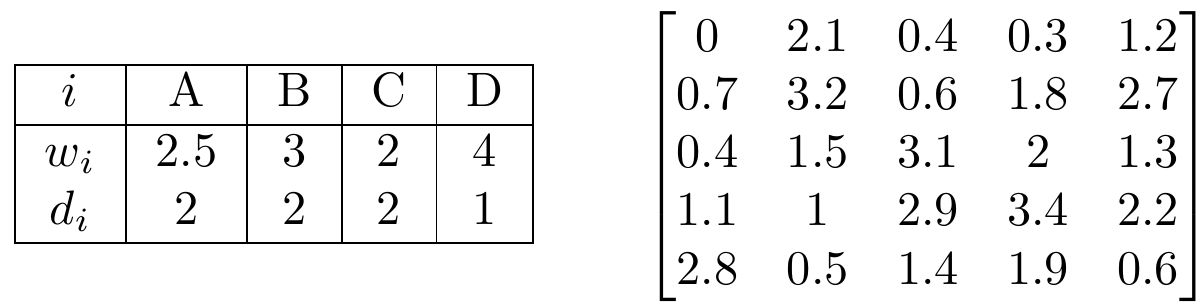
\includegraphics[width=\textwidth]{figures/sdcl5}
		\label{fig:sdcldemand}
	\end{subfigure} %
	\begin{subfigure}[h]{0.6\textwidth}
		\centering
		\includestandalone[width=\textwidth]{figures/sdcl}
		\label{fig:sdcl}
	\end{subfigure}	
	\caption{An example instance and solution for the CSP-SDCL showing the widths $w_i$ and demand $d_i$ for each item type $i$ and the cut losses matrix. The solution comprises three pieces of stock, where the lined areas are the cut losses and the remaining space on the end of each stock is shaded in grey. Here, $W = 10$.}	
	\label{fig:cspsdcl}
\end{figure}

%-------------------------------------------------------------------------------------

\subsection{The Strip Packing Problem}
\label{sub:spp}

\noindent The strip packing problem (SPP) is a two-dimensional packing problem classified as an open-dimensional problem by \citet{wascher2007}. Given a set $\mathcal{I}$ of $n$ rectangular items of varying heights $h_i \in \mathbb{Z}^+$ and widths $w_i \in \mathbb{Z}^+$ for all $i \in \mathcal{I}$, and a strip of fixed width $W$ and infinite height $H$, the problem involves packing the items onto the strip such that no items overlap and the height $H$ of the items on the strip is minimised.

Consider the bottom-left corner of the strip as the origin of the $xy$-plane, where the width of the strip is along the $x$-axis and the height of the strip is along the $y$-axis. Then, the coordinates $(x_i,y_i)$ represent the location of the bottom-left corner of each item $i \in \mathcal{I}$ on the strip. From this, we can formulate the SPP as follows:
\begin{subequations}
	\begin{align}
	\text{minimise  } &\qquad H  & \label{eq:objspp} \\[2pt]
	\text{subject to  } &\qquad x_i + w_i \leq W & i = 1,\dotsc,n \label{eq:capacitysppW}\\[2pt]
	&\qquad y_i + h_i \leq H & i = 1,\dotsc,n \label{eq:capacitysppH}\displaybreak[0]\\
	&\qquad x_i + w_i \leq x_j \text{ or } x_j + w_j \leq x_i \text{ or} & \nonumber \\
	&\qquad y_i + h_i \leq y_j \text{ or } y_j + h_j \leq y_j & i,j = 1,\dotsc,n, \hspace{1mm} i \neq j \label{eq:nooverlapspp} \\[2pt]
	&\qquad x_i, y_i \geq 0 & i = 1,\dotsc,n. \label{eq:allpackedspp}
	\end{align}
\end{subequations}

\noindent Clearly, the objective~\eqref{eq:objspp} is to reduce the overall height on the packing on the strip. Constraints~\eqref{eq:capacitysppW}, \eqref{eq:capacitysppH}, and~\eqref{eq:allpackedspp} impose the requirement for all items to be packed within the bounds $H\times W$ of the strip. Constraint~\eqref{eq:nooverlapspp} ensures that no items overlap \citep{kenmochi2009}.

The SPP is a generalisation of the BPP, where in the BPP all heights are equal; thus concluding that the SPP is also NP-hard. From the original problem, introduced by \citet{baker1980}, stems an abundance of adaptations developed for a variety of applications. One additional constraint to the SPP involves packing the items in their given orientations \citep{ntene2008}, whilst much literature exists for the SPP in which the rectangular items can be rotated $90^{\circ}$ -- see, for example, the works of \cite{jansen2005}, \citet{kenmochi2009}, \citet{cui2013}, and \citet{he2013}. An example of two solutions for an instance of the SPP with and without item rotations is provided in Figure~\ref{fig:spp}, showing that the ability to rotate the items can reduce the height of the packing. 

\begin{figure}[h!]
	\centering	
	\begin{subfigure}[h]{0.47\textwidth}
		\centering
		\includestandalone[width=0.73\textwidth]{figures/sppnorotation}
		\caption{}
		\label{fig:sppnorotation}
	\end{subfigure} %
	\begin{subfigure}[h]{0.47\textwidth}
		\centering
		\includestandalone[width=0.73\textwidth]{figures/spprotation}
		\caption{}
		\label{fig:spprotation}
	\end{subfigure}	
	\caption{Feasible solutions for an example instance of the SPP comprising 6 items. In (a) the items are packed in their given orientations, whilst in (b) the items can be rotated by $90^{\circ}$, resulting in a better packing.}	
	\label{fig:spp}
\end{figure}

\noindent Further constraints have been added to SPPs such as the ``guillotineable'' requirement, where items are to be packed onto the strip such that, at specific locations, a straight-line cut can be made across the width of the strip without cutting through an item as shown in Figure~\ref{fig:guillospp} \citep{kroger1995, hifi1998}. Other related problems include shelf divisions, in which items must be packed into subsections on the strip \citep{xavier2008}, and unloading constraints where the feasibility of the solution is dependent on the order of the items on the strip \citep{dasilveira2013}.

\begin{figure}[h!]
	\centering	
	\begin{subfigure}[h]{0.4\textwidth}
		\centering
		\includestandalone[width=0.6\textwidth]{figures/guillotine}
		\caption{}
		\label{fig:guillotine}
	\end{subfigure} %
	\begin{subfigure}[h]{0.4\textwidth}
		\centering
		\includestandalone[width=0.6\textwidth]{figures/nonguillotine}
		\caption{}
		\label{fig:nonguillotine}
	\end{subfigure}	
	\caption{Examples of (a) a guillotineable packing; and (b) a non-guillotineable packing.}	
	\label{fig:guillospp}
\end{figure}

%-------------------------------------------------------------------------------------

\section{The Score-Constrained Packing Problem}
\label{sec:scpp}

\noindent We now turn our attention to the Score-Constrained Packing Problem (SCPP). Let $\mathcal{I}$ be an instance of the SCPP, which contains $|\mathcal{I}| = n$ rectangular items of fixed height $H > 0$ and varying widths $w_i$ and score widths $a_i, b_i$ for each item $i \in \mathcal{I}$, as described in Definition~\ref{defn:scpp}. Then, given a minimum scoring distance $\tau \in \mathbb{Z}^+$, a feasible solution for an instance $\mathcal{I}$ of the SCPP is represented by the set $\mathcal{S} = \{S_1, S_2,\dotsc,S_k\}$ such that:
\begin{subequations}
	\begin{alignat}{2}
	\bigcup\nolimits_{j=1}^{k} S_j &= \mathcal{I}, & \label{eq:packall}\\[4pt]
	S_i \cap S_j &= \emptyset &\quad &i, j = 1,2,\dotsc,k, \hspace{1mm} i \neq j, \label{eq:nooverlap} \\[4pt]
	A(S_j) = \sum_{i=1}^{|S_j|}w_i &\leq W &\quad &j = 1,2,\dotsc,k, \label{eq:capacity} \\[4pt]
	\textup{\textbf{r}}(i) + \textup{\textbf{l}}(i+1) &\geq \tau &\quad &i = 1, 2,\dotsc,|S_j|-1, \hspace{1mm} j = 1,2,\dotsc,k. \label{eq:vscbin}
	\end{alignat}
\end{subequations}

\noindent In other words, the solution $\mathcal{S}$ must contain all items in $\mathcal{I}$ \eqref{eq:packall}, each item in $\mathcal{I}$ must be packed into exactly one of the bins in $\mathcal{S}$ \eqref{eq:nooverlap}, the total width of the items in each bin cannot exceed the bin's capacity $W$ \eqref{eq:capacity}, and the items must be arranged such that the vicinal sum constraint~\eqref{eq:vsc} is fulfilled in each bin \eqref{eq:vscbin}. Here, a bin $S_j \in \mathcal{F}$ if and only if Constraints~\eqref{eq:capacity} and \eqref{eq:vscbin} are satisfied. An optimal solution for the SCPP is a solution comprising the fewest number of bins required to feasibly pack all items in $\mathcal{I}$; thus the aim is to minimise the number of bins $k$. Observe that the BPP can be seen as a special case of the SCPP where $\tau = 0$, as the vicinal sum constraint will always be satisifed. As a result, the SCPP is also NP-hard.

As previously mentioned, there exists a basic lower bound $t$~\eqref{eq:tmin} for the number of bins $k$ in a solution for an instance of the BPP. However, this lower bound does not perform as accurately for the SCPP on account of the vicinal sum constraint. Consider an instance $\mathcal{I}$ of $n$ items in which the largest score width of all $2n$ score widths is less than $\tau/2$. Evidently, none of the items can be placed next to one another as there are no pairs of score widths that comply with the vicinal sum constraint. Under these circumstances, each item must be packed into individual bins; thus $k = n$. The theoretical minimum $t$ for the BPP does not take into consideration the effect of the minimum scoring distance $\tau$ on the feasibility of the solution. Therefore, a solution for an instance of the SCPP comprising more than $t$ bins could in fact be optimal, however as there is currently no appropriate lower bound for the SCPP it would be difficult to determine the optimality of a solution for large instances in a reasonable amount of time. Nevertheless, if a solution for an instance of the SCPP comprises exactly $t$ bins then the solution is guaranteed to be optimal.

In addition to the lower bound, the vicinal sum constraint also gives rise to further differences in solutions for the BPP and SCPP. Obviously, the main distinction involves the ordering and orienation of the items in the bins: inconsequential in the BPP, yet crucial for the feasibility of a solution for the SCPP. This subsequently introduces a disparity when amending solutions. A solution to the BPP remains feasible when an item is removed from a bin or when an item is added to a bin, provided the bin can accommodate the item. In contrast, this may render a solution for the SCPP infeasible as the new adjacent score widths may not satisfy the vicinal sum constraint.

In essence, the SCPP involves deciding (a) which items should be packed into which bins and (b) the order and orientation of each item within each bin. This problem characteristic also occurs in two of the problems discussed in the previous section, namely the TPP and the CSP-SDCL. One particular difference, however, between these problems and the SCPP concerns the feasibility of individual bins. For example, in the TPP it is still possible to pack trapezoids with opposite angles, i.e. `$\backslash$' and `/', alongside one another, despite the unnecessarily large inter-item waste. Similarly, in the CSP-SDCL two items with a large cut loss between them can still be packed alongside one another if required. Both of these packing problems permit \emph{any} order and orientation of items provided the bins are not overfilled. Conversely, the SCPP possesses the strong vicinal sum constraint, which if violated immediately causes an alignment of items in a bin to be invalid, rendering the entire solution infeasible.

To illustrate the differences between the BPP and the SCPP, suppose we use items for an instance $\mathcal{I}$ of the SCPP in the previous BPP solution in Figure~\ref{fig:bppsoln}, as shown in Figure~\ref{fig:bppvscpp}.\footnote{Note that the SCPP instance $\mathcal{I}$ used in Figure~\ref{fig:bppvscpp} is the instance depicted in Figure~\ref{fig:scppitems} in Chapter~\ref{chap:intro}, which is equivalent to the BPP instance in Figure~\ref{fig:bppitems} with added score widths.} Note that the BPP solution is actually produced using the FFD heuristic described in Section~\ref{sec:heurbpp}. As the vicinal sum constraint is not a factor in the BPP and the FFD heuristic does not have the ability to rotate items, all the items are packed into the bins in regular orientations (i.e. with the smallest score width on the left-hand side of the item). Despite using fewer bins, the solution produced for the BPP is not feasible for the SCPP; the vicinal sum constraint is violated at least once in every bin. Furthermore, the theoretical minimum for the instance $\mathcal{I}$ is $t=3$ which is attainable for the conditions of the BPP (for example, if $\tau = 0$) however, for the SCPP it is known that for this particular instance an optimal solution comprises four bins.

\begin{figure}[h!]
	\centering	
	\begin{subfigure}[h]{0.6\textwidth}
		\includestandalone[width=\textwidth]{figures/bppscores}
		\caption{BPP}
		\label{fig:bppscores}
		\vspace{5mm}
	\end{subfigure} 
	\begin{subfigure}[h]{0.6\textwidth}
		\includestandalone[width=\textwidth]{figures/scpp}
		\caption{SCPP}
		\label{fig:scppscores}
	\end{subfigure}
	\caption{A comparison of solutions for the BPP and SCPP using the same problem instance for the SCPP, where the red score lines on the BPP solution show the vicinal sum constraint violations. Here, $|\mathcal{I}| = 10$, $\tau = 70$, and $W = 1000$.}	
	\label{fig:bppvscpp}
\end{figure}

\noindent Evidently, basic methods designed for the BPP cannot be used for the SCPP as there is no guarantee that the final solution will be feasible. The disparities between the BPP and SCPP leads us to adapt existing methods and seek new unique approaches capable of producing feasible solutions that adhere to the constraints of the SCPP.

%-------------------------------------------------------------------------------------

\section{Computational Complexity}
\label{sec:complexity}

\noindent To begin, let us distinguish between two types of problem.

\begin{definition}
	A \emph{decision problem} is a problem in which the answer is either ``yes'' or ``no'', depending on the input. An \emph{optimisation problem} is a problem where an optimal solution is to be found from all feasible solutions, with respect to some given objective function.
	\label{defn:problems}
\end{definition}

\noindent Observe that optimisation problems can be transformed into decision problems and vice versa. Consider, for example, the travelling salesman problem (TSP). The optimisation variant of the problem is: ``find the tour with the shortest length'', whilst the decision variant is: ``for each value $D$, does there exist a tour with length less than $D$?''. It can be seen that if the decision problem is asked and answered repeatedly, the length of the shortest tour can be determined. 

The field of computational complexity theory concentrates on classifying problems into distinct complexity classes, which allows us to compare the difficulty of different problems. The classification of a problem is determined by the number of machine operations, or running time, needed by an algorithm to find or verify a solution to the problem relative to the input size.

An algorithm is said to be of \emph{polynomial-time} if its running time is upper-bounded by a polynomial expression in terms of the input size for the algorithm. Such algorithm are considered to be efficient algorithms \citep{edmonds1965, cobham1965}. Consequently, a problem is said to be \emph{polynomial} if there exists a polynomial-time algorithm for finding a solution for any instance of the problem. The complexity class P contains all polynomial decision problems. One other way of describing P is that the decision problems in P can be solved by a \emph{deterministic} Turing machine.

There are many problems for which no polynomial-time algorithms for finding solutions have yet been found. Unfortunately, it has also not been determined that there do not exist polynomial-time algorithms for such problems. For some of these problems, however, it is possible to \emph{verify} a solution in a reasonable amount of time. A problem is said to be \emph{non-deterministic polynomial} if there exists a polynomial-time algorithm that is able to verify any given solution to the problem \citep{cook1971}. The complexity class NP contains all non-deterministic polynomial decision problems. Again, NP can be described as the set of decision problems for which a given solution can be verified in polynomial-time by a deterministic Turing machine, or that is solvable by a \emph{non-deterministic} Turing machine in polynomial-time. Clearly, as non-deterministic Turing machines are theoretical, it is thought that problems in NP will always be intractable to solve with our regular (deterministic) machines; thus, is it widely assumed that P$\neq$NP.

A problem is said to be NP-hard if every problem in NP can be reduced by a polynomial-time algorithm into that problem. Note, however, that NP-hard problems do not have to be in NP and may not even be decision problems -- they can also be optimisation or search problems. On the other hand, a problem is said to be NP-complete if it is NP-hard \emph{and} is an element of NP. NP-complete problems are considered to be the hardest problems in NP, whilst NP-hard problems are at least as hard as the problems in NP-complete. Therefore, if there exists a polynomial-time algorithm that can \emph{solve} an NP-hard problem it would then be possible to solve all problems in NP in polynomial-time, and so P=NP.  Figure~\ref{fig:complexity} illustrates the relationship between these complexity classes assuming P$\neq$NP. 

Many surveys, articles, and books covering computational complexity theory are readily available, including overviews on the topic \citep{cook1983}, pioneering work on NP-completeness \citep{karp1972}, discussions into the importance of considering the equality of P and NP \citep{cook2006}, as well as general books exploring various aspects of the field \citep{garey1979, papadimitriou2003}. In addition, further information on Turing machines can be found in the notable works of \citet{petzold2008} and \citet{jongen2007}.

\begin{figure}[h!]	
	\centering
	\includestandalone[width=0.45\textwidth]{figures/complexity}
	\caption{A diagram showing the relationship between the complexity classes P, NP, NP-hard, and NP-complete under the assumption that P$\neq$NP.}	
	\label{fig:complexity}
\end{figure}

%-------------------------------------------------------------------------------------

\section{Grouping Problems}
\label{sec:groupingprobs}

\noindent Many combinatorial optimisation problems involve the grouping or partitioning of elements into subsets. These types of problems can be seen in areas such as scheduling \citep{thompson1998, carter1996}, frequency assignment \citep{aardal2007}, graph colouring \citep{lewis2012, malaguti2008}, and load balancing \citep{rekiek1999}, as well as in practical problems in computer science such as table formatting, prepaging, and file allocation \citep{garey1972}. Formally, given a set $\mathcal{I}$ of $n$ elements, the aim is to produce a set of groups $\mathcal{S} = \{S_1, S_2,\dotsc,S_k\}$ such that:
\begin{subequations}
	\begin{alignat}{2}
	\qquad \qquad \bigcup\nolimits_{j=1}^{k} S_j &= \mathcal{I}, & \quad \label{eq:allpacked}\\[3pt]
	S_i \cap S_j &= \emptyset &\quad &i, j = 1, 2,\dotsc,k, \hspace{1mm} i \neq j, \label{eq:nointersect}\\[3pt]
	S_j &\in \mathcal{F} &\quad &j = 1,2,\dotsc,k.\label{eq:feasible}
	\end{alignat}
\end{subequations}

\noindent Conditions~\eqref{eq:allpacked} and~\eqref{eq:nointersect} enforce the requirement that every element in $\mathcal{I}$ must be in exactly one of the $k$ groups in $\mathcal{S}$, whilst Condition~\eqref{eq:feasible} specifies that each group $S_j \in \mathcal{S}$ must be \emph{feasible}. Here, we introduce the set $\mathcal{F}$, which denotes the set of all feasible subsets of elements in $\mathcal{I}$. The notion of feasibility is dependent on the particular constraints of the given problem. 

The graph colouring problem (GCP) involves assigning colours to vertices on a graph $G$ such that no two adjacent vertices are of the same colours, with the objective of minimising the total number of colours used. The chromatic number of a graph $G$, denoted $\chi(G)$, is the minimum number of colours required to colour $G$. The GCP is one example of a grouping problem, where the vertices of the graph must be grouped into the fewest non-overlapping subsets (i.e. colour classes) such that each subset is an independent set. For this problem, $\mathcal{F}$ contains all possible independent sets of vertices on the graph. Figure~\ref{fig:gcp} illustrates an example solution of the GCP on a graph $G$ comprising eight vertices, where $\chi(G) = 4$ colours have been used to colour the vertices feasibly. For a deeper introduction to graph colouring, the reader is directed to the work of \citet{lewis2015}.

Another example of a grouping problem occurs when scheduling exams in schools and universities. In its simplest form, the problem involves sorting exams into a limited number of timeslots whereby no student is scheduled to sit more than one exam per timeslot. In practice, however, many other factors must be considered such as the exam locations, the capacity of each location, and restrictions on the order of specific exams. For this problem, each timeslot can be considered as a group; thus $\mathcal{F}$ contains all possible groups of exams where each student is attending at most one exam.

It is interesting to note that the exam scheduling problem can in fact be reformulated as a graph colouring problem. Suppose each exam $i$ is represented by a vertex $v_i$ on a graph $G$, and for each pair of exams $i$ and $j$ there exists an edge $\{v_i, v_j\}$ on $G$ if at least one student is required to sit both exams. Then, the resulting graph $G = (V, E)$ depicts the exams than can and cannot be scheduled into the same timeslot. By finding a solution to the GCP with respect to $G$, the fewest number of timeslots for which all exams can be scheduled without clashes can be determined. Figure~\ref{fig:exams} shows the number of students required to sit each pair of exams for the subjects \textbf{Al}gebra, \textbf{An}alysis, \textbf{C}alculus, \textbf{G}eometry, \textbf{M}echanics, \textbf{N}umber Theory, \textbf{O}ptimisation, and \textbf{S}tatistics. The colours of the vertices on the graph $G$, shown in Figure~\ref{fig:gcp}, indicate the exams that should be scheduled into the same timeslots.

\begin{figure}[h!]
	\centering	
	\begin{subfigure}[b]{0.4\textwidth}
		\includestandalone[width=\textwidth]{figures/exams}
		\caption{}	
		\label{fig:exams}
	\end{subfigure} \hspace{5mm}
	\begin{subfigure}[b]{0.4\textwidth}
		\includestandalone[width=\textwidth]{figures/gcptimetable}
		\caption{}	
		\label{fig:gcp}
	\end{subfigure}
	\caption{(a) An example instance of the exam scheduling problem, where the table shows for each pair of subjects the number of students sitting both exams; and (b) the graph $G$ depicting the scheduling problem. Solving the GCP on $G$ shows that four timeslots are required, with the vertex colours indicating the exams that should be assigned to the same timeslot.}	
	\label{fig:groupingprobs}
\end{figure}

\noindent A grouping problem will often have one of two objectives regarding the number of groups $k$ in a solution $\mathcal{S}$. One objective involves determining whether a solution $\mathcal{S}$ exists that contains exactly $k$ groups, where $k$ has been explicity specified. Grouping problems with this type of objective are decision problems. The other objective is to find a solution comprising the fewest number of groups $k$; these types of grouping problems are optimisation problems. This latter class of problems, identified by \citet{lewis2011} as Minimum Grouping Problems (MGPs), can be separated into two sub-classes: Order Dependent Minimum Grouping Problems (ODMGPs), where the order of the groups affects the feasibility and/or quality of the solution -- for example, the exam scheduling problem with an additional condition preventing students from sitting exams in consecutive timeslots -- and Order Independent Minimum Grouping Problems (OIMGPs), in which the order of the groups within a solution is irrelevant. 

%-------------------------------------------------------------------------------------

\section{Summary}
\label{sec:litsummary}

\noindent In this chapter, we introduced grouping problems and focused on a particular class of such problems known as cutting and packing problems. The one-dimensional bin packing problem (BPP) was presented and shown to be NP-hard, implying that finding optimal solutions for larger problem instances can take an infeasible amount of time. From this, we discussed various approaches to the BPP such as heuristics and metaheuristics which find near-optimal solutions in a more practical time period, as well as a few exact methods that are suitable for smaller, more manageable problem instances. The BPP was also shown to give rise to numerous alternative cutting and packing problems that have been adapted to suit a range of applications.

By reviewing the BPP, we were able to observe the similarities and differences between the BPP and the Score-Constrained Packing Problem (SCPP), and deduce that the SCPP is also NP-hard. The most notable contrast is the ordering and orientation implications associated with the SCPP, indicating that methods available for the BPP are incompatible with the SCPP. Consequently, the remainder of this thesis is devoted to constructing algorithms for the SCPP that yield high quality feasible solutions.

Recall that for the TPP -- another packing problem involving the ordering and orientation of items (see Section~\ref{sec:variationsbpp}) -- the authors developed an exact polynomial-time algorithm for determining a feasible alignment of items in a single bin. Following on in a similar manner, the next chapter presents an algorithm for the Score-Constrained Packing Sub-Problem (sub-SCPP) introduced in Definition~\ref{defn:subscpp}.

\bibliographystyle{plainnat}
\bibliography{includes/bibliography}

\end{document}